\documentclass[12pt,oneside]{book}
\usepackage{times,mathptmx}
\usepackage[pdftex]{graphicx}
\usepackage{calc}
\usepackage{tabularx,ragged2e,booktabs,caption,subcaption}
\usepackage{array}
\newcolumntype{L}[1]{>{\raggedright\let\newline\\\arraybackslash\hspace{0pt}}m{#1}}
\newcolumntype{C}[1]{>{\centering\let\newline\\\arraybackslash\hspace{0pt}}m{#1}}
\newcolumntype{R}[1]{>{\raggedleft\let\newline\\\arraybackslash\hspace{0pt}}m{#1}}
\usepackage{multirow}
\usepackage{tocloft}
\usepackage{xcolor}
\usepackage{color,soul}
\usepackage{amsmath}
\definecolor{linknavy}{rgb}{0,0,0.50196}
\definecolor{linkred}{rgb}{1,0,0}
\definecolor{linkblue}{rgb}{0,0,1}
\usepackage{float}
\usepackage{graphpap}
\usepackage{rotating}
\usepackage{graphicx}
\usepackage{geometry}
\usepackage{relsize}
\usepackage{ltablex}
\usepackage{longtable}
\usepackage{lscape}
\usepackage{amssymb}
\usepackage{makeidx} % Create index at end of document
\usepackage[nottoc,notlof,notlot]{tocbibind} % Put the bibliography and index in the ToC
\usepackage{lastpage} % Automatic last page number reference.
\usepackage[T1]{fontenc}
\usepackage{enumerate}
\usepackage{upquote}
\usepackage{moreverb}
\usepackage{xfrac}
\usepackage{cite}
\usepackage{tikz}
% \usepackage{subfig}
% \usepackage{caption}
\usepackage[toc,page]{appendix}
\usepackage{notoccite}
\usepackage{colortbl}
\usepackage{titlesec}
\titleformat{\chapter}[hang] 
{\normalfont\huge\bfseries}{\chaptertitlename\ \thechapter}{1em}{} 
\titlespacing*{\chapter}{0pt}{-30pt}{20pt}

\newcommand{\nopart}{\expandafter\def\csname Parent-1\endcsname{}} % To fix table of contents in pdf.

\usepackage{siunitx}
\sisetup{
    detect-all = true,
    input-decimal-markers = {.},
    input-ignore = {,},
    inter-unit-product = \ensuremath{{}\cdot{}},
    multi-part-units = repeat,
    number-unit-product = \text{~},
    per-mode = fraction,
    separate-uncertainty = true,
}

\usepackage{listings}
\usepackage{textcomp}
\definecolor{lbcolor}{rgb}{0.96,0.96,0.96}

\usepackage[pdftex,
        colorlinks=true,
        urlcolor=linkblue,     % \href{...}{...} external (URL)
        citecolor=linkred,     % citation number colors
        linkcolor=linknavy,    % \ref{...} and \pageref{...}
        pdfproducer={pdflatex},
        pdfpagemode=UseNone,
        bookmarksopen=true,
        plainpages=false,
        verbose]{hyperref}

\setlength{\textwidth}{6.5in}
\setlength{\textheight}{9.0in}
\setlength{\topmargin}{0.in}
\setlength{\headheight}{0.pt}
\setlength{\headsep}{0.in}
\setlength{\parindent}{0.0in}
\setlength{\itemindent}{0.25in}
\setlength{\oddsidemargin}{0.0in}
\setlength{\evensidemargin}{0.0in}
% \setlength{\leftmargini}{\parindent} % Controls the indenting of the "bullets" in a list
\setlength{\cftsecnumwidth}{0.45in}
\setlength{\cftsubsecnumwidth}{0.5in}
\setlength{\cftfignumwidth}{0.45in}
\setlength{\cfttabnumwidth}{0.45in}
\setlength{\parskip}{1em}

\newcommand{\titlesigs}
{
\large
\flushright{UL Firefighter Safety Research Institute\\
{\em Stephen Kerber, Director} \\
\hspace{1in} \\
}
}

\newcommand{\headerB}[1]{
\flushleft{
\fontsize{28}{33.6}\selectfont
\bf{#1}
}
}

\newcommand{\headerC}[1]{
\vspace{.5in}
\flushright{\fontsize{14}{16.8}\selectfont
#1}
}

% \newcolumntype{L}{>{\centering\arraybackslash}m{4cm}}

\floatstyle{boxed}
\newfloat{notebox}{H}{lon}
\newfloat{warning}{H}{low}

\newenvironment{conditions}
  {\par\vspace{\abovedisplayskip}\noindent\begin{tabular}{>{$}l<{$} @{${}={}$} l}}
  {\end{tabular}\par\vspace{\belowdisplayskip}}


\usepackage{pdflscape}
\usepackage{longtable}
\usepackage{fancyhdr}
\usepackage{everypage}

\pagestyle{fancy}
\lhead{}
\rhead{}
\chead{}
\renewcommand{\headrulewidth}{0pt}

\newcommand{\Lpagenumber}{\ifdim\textwidth=\linewidth\else\bgroup
  \dimendef\margin=0
  \ifodd\value{page}\margin=\oddsidemargin
  \else\margin=\evensidemargin
  \fi
  \raisebox{\dimexpr -\topmargin-\headheight-\headsep-0.5\linewidth}[0pt][0pt]{%
    \rlap{\hspace{\dimexpr \margin+\textheight+\footskip}%
    \llap{\rotatebox{90}{\thepage}}}}%
\egroup\fi}
\AddEverypageHook{\Lpagenumber}%

\setcounter{secnumdepth}{0}

\begin{document}
\pagenumbering{gobble}

\frontmatter

\begin{minipage}[t][9in][s]{6.25in}

\headerB{\ul{
Tech Panel Comments \& Responses
}}

\vspace{0.5in}

\headerB{
Impact of Fire Attack Utilizing \\
Interior and Exterior Streams on\\ 
Firefighter Safety and Occupant \\
Survival: Water Mapping\\
}

\vspace{1.5in}

\today

\normalsize

\headerC{
{
\flushleft{
\vspace{0.2in}
Craig Weinschenk \\
Keith Stakes \\
Robin Zevotek \\
UL Firefighter Safety Research Institute \\
Columbia, MD 21045 \\
\vspace*{2\baselineskip}

}

\vfill

\flushright{


\includegraphics[width=2.in]{Figures/General/FSRI_GraphicShield} \\[.3in]
}
}
}
\end{minipage}

\newpage

\tableofcontents

\newpage

\mainmatter

\chapter*{Background}
\label{background}
\addcontentsline{toc}{chapter}{\nameref{background}}

This document has been created to track and respond to the comments made by the technical panel as part of the UL FSRI DHS 2013 project "Impact of Fire Attack Utilizing Interior and Exterior Streams on Firefighter Safety and Occupant Survival: Water Mapping". 

A special thanks to the individuals listed below who provided feedback to the project team at FSRI, in addition to the information contained in this document we also received emails that said they had no comments along with many phone calls where we answered questions as well.  Thank you all for the engagement. 

\begin{table}[!ht]
	\centering
	\caption*{Fire Service Technical Panel}
	\begin{tabular}{lc}
		\toprule[1.5pt]
		Name & Fire Department \\ 
		\hline
		Steve Brisebois  & Montreal Fire Department \\ 
		Matt Carrigan    & Montgomery County Fire and Rescue Service \\ 
		Tony Carroll     & Washington DC Fire Department \\ 
		Albert Castillo  & Houston Fire Department \\ 
		Chad Christensen & Los Angeles County Fire Department \\ 
		John Chubb       & Dublin Fire Brigade \\ 		 		  
		Danny Doyle      & Pittsburgh Fire Department \\ 
		Aaron Fields     & Seattle Fire Department \\ 
		Jason Floyd      & Las Cruces Fire Department \\ 
		John Gallagher   & Boston Fire Department \\ 
		Chad Green       & Anchorage Fire Department \\ 
		Kelly Hanink     & Eden Prairie Fire Department \\ 
		Samuel Hittle    & Wichita Fire Department \\ 
		Jacob Hoffman    & Toledo Fire/Rescue Department \\ 
		Josh Hummel      & Howard County Department of Fire and Rescue Services \\ 
		Jerry Knapp      & West Haverstraw (NY) Fire Department \\ 
		Dennis Legear    & Oakland Fire Department \\ 
		Hans Neiling     & Zuid Limburg Fire \\ 
		Nick Martin      & Columbia Fire Department \\ 
		Ray McCormack    & Fire Department of New York \\ 
		John McDonough   & New South Wales Fire Department \\ 
		Jordan Mohr      & Sedgwick County Fire District 1 \\ 
		Steve Pegram     & Goshen Township Fire and EMS \\ 
		\bottomrule[1.25pt]
	\end{tabular}
\end{table}

% \begin{table}[!ht]
% 	\centering
% 	\caption*{Fire Service Technical Panel}
% 	\begin{tabular}{llc}
% 		\toprule[1.5pt]
% 		& Name & Fire Department \\ 
% 		\hline
% 		& Steve Brisebois  & Montreal Fire Department \\ 
% 		& Matt Carrigan    & Montgomery County Fire and Rescue Service \\ 
% 		& Tony Carroll     & Washington DC Fire Department \\ 
% 		& Albert Castillo  & Houston Fire Department \\ 
% 		\checkmark & Chad Christensen & Los Angeles County Fire Department \\ 
% 		& John Chubb       & Dublin Fire Brigade \\ 		 		  
% 		& Danny Doyle      & Pittsburgh Fire Department \\ 
% 		& Aaron Fields     & Seattle Fire Department \\ 
% 		\checkmark & Jason Floyd      & Las Cruces Fire Department \\ 
% 		& John Gallagher   & Boston Fire Department \\ 
% 		& Chad Green       & Anchorage Fire Department \\ 
% 		\checkmark & Kelly Hanink     & Eden Prairie Fire Department \\ 
% 		& Samuel Hittle    & Wichita Fire Department \\ 
% 		\checkmark & Jacob Hoffman    & Toledo Fire/Rescue Department \\ 
% 		\checkmark & Josh Hummel      & Howard County Department of Fire and Rescue Services \\ 
% 		\checkmark & Jerry Knapp      & West Haverstraw (NY) Fire Department \\ 
% 		\checkmark & Dennis Legear    & Oakland Fire Department \\ 
% 		\checkmark & Hans Neiling     & Zuid Limburg Fire \\ 
% 		& Nick Martin      & Columbia Fire Department \\ 
% 		\checkmark & Ray McCormack    & Fire Department of New York \\ 
% 		& John McDonough   & New South Wales Fire Department \\ 
% 		\checkmark & Jordan Mohr      & Sedgwick County Fire District 1 \\ 
% 		& Steve Pegram     & Goshen Township Fire and EMS \\ 
% 		\bottomrule[1.25pt]
% 	\end{tabular}
% 	\\ \checkmark~~indicates panel member provided feedback on the water mapping report.
% \end{table}

\newpage



\chapter*{Comments and Responses}
\label{comments}
\addcontentsline{toc}{chapter}{\nameref{comments}}
In general it seems the use of ``Interior'' and ``Exterior'' have caused some significant challenges for interpreting the results. We've heard the concerns and thus have changed the terminology in the report to reflect this. All instances where the application of water through a window was tested is not referenced as a ``Window Attack'' and all references where water through a doorway was tested is referenced as a ``Doorway Attack''. The objectives in section 2 and the test descriptions in section 3.2 have been adjust to provide a better description of the intent of the testing. These tests were designed to develop a fundamental understand of where water goes after leaving a hose stream, and is applied into compartments. It was not intended to test the ability of our team to point a nozzle in a particular direction and hit a target. 

It is understood that once a room, a firefighter can put water anywhere in the room by moving the nozzle or their body.  This is completely within the control of the firefighter.  When outside the room this is not possible and we wanted to show the limitations of water application when outside the room. Once we understand the dynamics of water hitting a surface at different angles we can extrapolate to other locations.  For example, flowing wall ceiling wall going down the hallway allows little water to enter the compartment because the bulk of the water rides the walls and does not bounce off the wall and into the compartment.  In some fires that may be enough and in others you may need to direct the nozzle straight in through the room but once you do that...we know most of the water goes along the back wall which means you need to get into the compartment to extinguish the fire.   

We have adjusted the tactical choices summary to include specific information about this. Please read through and let us know if we've addressed your specific comments. \textbf{If you still feel we need more clarification please provide the text you'd like to see in the document.}

The following tables capture the comments from technical panel members, the response from FSRI and if the report has been updated. The fist column is the comment, often copied directly from e-mails received from the panel member. The second column is the FSRI response to the comment. \textbf{Where FSRI is requesting clarity the questions are in bold font.} If the report was changed based on the comment a \checkmark is located in the third column. 
\begin{landscape}

\pagestyle{empty}
\section{Chad Christensen}
% \section{Responder 1}
\begin{longtable}{|L{4in}|L{3.75in}|c|}

		\hline
		Comment/Question & Response & Report Update \\ 
		\toprule[1.0pt] \endfirsthead
		\hline
		Comment/Question & Response & Report Update \\ 
		\toprule[1.0pt] \endhead
		\hline
		Is their any CO data for test 3? It says the sensors were not used? Is the data just not loaded yet or was that the burn they were having sensor issues. Sorry can't remember! &
		Comment pertains to fire attack report data, will answer when we get to fire experiment review. & \\
		
		\hline
		If I am reviewing things with an open mind and trying to be objective am I correct in that the temps with door control incorporated drop at a quicker rate than without? Between test 2 and 3? & 
		Comment pertains to fire attack report data, will answer when we get to fire experiment review. & \\

		\hline
		Overall it also appears that water on the fire regardless of how it was applied improved conditions in the fire room and surrounding areas. Yet the straight stream seems to be most effective. Early water on the fire appears to be best for the victims inside. &
		Comment pertains to fire attack report data, will answer when we get to fire experiment review. & \\

		\hline
		CO levels have been a big concern with guys when it comes to door control. Unless I am missing something it seems at least in my first glance, that CO levels in the survivable space are not raising until suppression? Are we making things worse by putting out the fire? It also seems that with door control CO levels didn't rise any more than without? & 
		Comment pertains to fire attack report data, will answer when we get to fire experiment review. & \\

		\hline
		To determine the best flow type is the velocity what we should be looking at? & 
		Comment pertains to fire attack report data, will answer when we get to fire experiment review. & \\

		\hline
\end{longtable}
\checkmark~~indicates change made to report to address comment.

\newpage

\section{Kelly Hanink}
% \section{Responder 2}
\begin{longtable}{|L{4in}|L{3.75in}|c|}

		\hline
		Comment/Question & Response & Report Update \\ 
		\toprule[1.0pt] \endfirsthead
		\hline
		Comment/Question & Response & Report Update \\ 
		\toprule[1.0pt] \endhead
		\hline

		\hline
		Figure 5.1 (pg 48) and its associated write-up don't seem to connect exactly. I had to re-read that piece and look at the picture again to understand it. The text states that the dispersion was fairly equally radially to 360 deg with some impact by gravity. But the horizontal arrows (at 90 and 270 deg) are nearly the same as the downward one (280 deg). I just think the arrows need to be depicted a little more accurately to match the words. & 
		Adjusted arrows to ensure the effect of gravity is better depicted. & \checkmark \\  

		\hline
		When I read the write-up about Figure 5.2 (pg 49) I thought it was lacking info, which it turns out I found in the section on water distribution in the next section. I don't know if it would be helpful to add text to the water dispersion paragraph to tell the reader about the additional effects of the high angle attack that are described further in the water distribution section or not. That might not be a thing needed in a research report. & 
		Section 5.2 is intended to discuss the dispersion (how the stream breaks up) and section 5.3 discusses how dispersion effects distribution. The idea is to provide building blocks for the reader to put together the pieces. \textbf{Please provide text to help further clarify.} & \\

		\hline
		I feel like the last two rows Table 5.1 (Tactical Choices Summary) present issues. The Nozzle Movement tactical choice states a positive impact for Interior attack from an `O' pattern at the ceiling. But the prior discussion about nozzle movement says "When compared to each other, nozzle movement had little effect on the distribution in the compartment... While the distribution for the fixed pattern was more uniform (flatter)..." Those statements don't appear to match. Further, in the nozzle movement discussion section, there doesn't seem to be any mention of nozzle movement and fog nozzles or any graphs that support the statement in the summary table that an `O' pattern provides good distribution. Or if there is, I didn't make the connection very well so you might want to look to see where things might be restated or tied together better. &
		Changed Nozzle movement to the following ``Nozzle movement had little effect on distribution.'' & \checkmark \\

		\hline 
		Table 5.1 In the Bale Position section, I don't think it's stated that the testing was only tested in the exterior case. Maybe that should be added to help with clarity and completeness and to support the last row of the summary table? &
		Added verbiage to Section 5.5.2 under bale position to indicate the expected interior results and adjusted table to match. & \checkmark \\  

		\hline
\end{longtable}
\checkmark~~indicates change made to report to address comment.

\newpage

\section{Josh Hummel}
% \section{Responder 3}
\begin{longtable}{|L{4in}|L{3.75in}|c|}

		\hline
		Comment/Question & Response & Report Update \\ 
		\toprule[1.0pt] \endfirsthead
		\hline
		Comment/Question & Response & Report Update \\ 
		\toprule[1.0pt] \endhead
		\hline
		I think it's important to include that these findings are purely distribution and not considering air entrainment so conclusions are drawn prematurely by those reading the study. (This could include the 1/2 bale smooth bore technique discussed at the end or even changing the angle of the stream in the window as it relates to air entrainment. I'm not sure if these were all tested in the entrainment piece or not) I can say that I wouldn't have drawn those conclusions as I'm reading the report for what it is, but could see it being a potential issue. & 
		Agreed, added the following paragraph to the end of the discussion section to address. ``This section discusses the tactical choices as they relate to water distribution. It is important to understand that water distribution is not the only concern when discussing fire suppression tactical choices. Other considerations, for example air entrainment, may play a role in the nozzle firefighters choice of hose stream. Fire suppression operations involve a significant number of variables, making the system extremely complex. Understanding how the variables interact is out of the scope of this particular analysis and discussion.'' & \checkmark \\

		\hline
		`bale' of a nozzle instead of `bail' & 
		IFSTA references `bale', changed all instances to match. & \checkmark \\

		\hline
		`Freeman' has typo as `Freedman' & 
		Corrected typo. & \checkmark \\

		\hline
\end{longtable}
\checkmark~~indicates change made to report to address comment.

\newpage

\section{Dennis Legear}
% \section{Responder 4}
\begin{longtable}{|L{4in}|L{3.75in}|c|}
		
		\hline
		Comment/Question & Response & Report Update \\ 
		\toprule[1.0pt] \endfirsthead
		\hline
		Comment/Question & Response & Report Update \\ 
		\toprule[1.0pt] \endhead
		\hline
		Page 4 - Is efficient in paragraph two tied to the amount of water used &
		This is a generic background discussion on fire attack. Efficient in this case means not only the water used but things such as the time it takes, amount of damage created or even the manpower needed. & \\
		
		\hline
		Having no floor in the test apparatus ``stops nozzle advancement into fire compartment, very unrealistic'' & 
		This set of tests was intended to evaluate where water is disturbed from fire service hoses when the nozzle firefighter cannot see through the smoke to determine what is on fire. The report does not suggest that water should not be put on fire, nor is it a complete evaluation of how to apply water into compartments. It is intended to develop a fundamental knowledge base where practical application incorporates all the principals derived from the results. & \\

		\hline
		``The goal of making the interior compartment in nozzle in the room where water application to all surface and furniture is possible bread and butter of interior attack *why I push for 2-story burns and stated in planning NO NOZZLE ALLOWED THROUGH WINDOWS'' & 
		We've addressed the interior/exterior issue in the general comments on page 2. The intent of the interior experiments is discussed in section 3.2.1. During this round the nozzle did not extend through the window. The results of this report are comparing the nozzle at the window (not inside) to the nozzle at the door (not inside). We have clarified this in Section 2, which describes the intended research as follows ``The the experiments conducted were intended to develop a fundamental knowledge of water distribution in compartments from fire service hose streams. After development, this knowledge can be extrapolated to the infinite number of scenarios in which the fire service may be applying water. The choices of stream location were developed to achieve this objective while at the same time simulating common fireground tactics. Due to the limitations of the equipment used and the force resulting from the application of water with common fire service hoses, directing the hose stream at the collection appliance was not possible nor would it produce a reliable and realistic measurement.'' additionally we've clarified the interior position to be ``the location at which you would cool the fire compartment before entering for final suppression'' in section 3.2.1 & \checkmark\\

		\hline
		Table 3.1 - Correct to common printed flows with nozzle pressure & 
		Corrected flow rate to match $29.7d^2\sqrt{P}$ with a 50~psi nozzle pressure for all smooth bore nozzles. Adjusted figures at the end to include correct flow rates. & \checkmark \\

		\hline
		Figure 3.7 - ``This turn a inter door into an exterior attack fixed position'', ``Very misleading a interior nozzle would only be in this position momentarily on advance maybe flowing maybe not flowing'' &
		We've addressed the interior/exterior issue in the general comments on page 2. The nozzle prop in the picture was constructed to limit the variability in the nozzle position throughout the tests, providing repeatability. The tests were designed as described in 3.2.1, with the position chosen to remove the impact of the soffit and or doorway on results. The specific position was chosen as the closest the nozzle team could get to the compartment, to apply water to the compartment without entering it. We have addressed the interior/exterior comment in section 3.2.1 and section 2. \textbf{Do you feel this needs further clarification} & \\

		\hline
		Section 3.2.1, ``Suppression operations were conducted from the doorway adjoining the hallway to the test compartment.'' ``max angle ceiling, mid ceiling, at wall''- We talked about the dry wall in planning clearly stated the goal was nozzle past door threshold of fire compartment. &
		We've addressed the interior/exterior issue in the general comments on page 2. The technical panel members present did not indicate this being a concern during testing. We revisited the notes from the planning meeting and did not see a reference to this.  We have addressed the interior/exterior comment in section 3.2.1 and section 2 & \\

		\hline
		Section 4 - ``application locations'' none a true interior attack in room bread and butter - knock with reach of stream/cool advance into room for base fire extinguishment no risk of regrowth. & 
		We've addressed the interior/exterior issue in the general comments on page 2. & \\

		\hline
		Figure 4.2 - Nozzle outside the room. This is not an interior attack until the nozzle moves FWD. A interior attack as submitted and discussed at the is to get the nozzle through the door threshold. & 
		This image is being shown to identify the direction the water was coming from. \textbf{If it does not depict this clearly, please provide text to help resolve.} & \\

		\hline
		Section 4.2 ``For the interior tests, both the fixed pattern and `O' pattern showed statistical differences'' Never entered the room gold standard. &
		We've addressed the interior/exterior issue in the general comments on page 2. & \\

		\hline
		Figure 4.3 - This is obvious and why nozzle must cross the threshold to gain access to properly coat room \& drywall \& full ceiling. &
		The goal of this phase of research was to look at how the water disperses in the room. Moving the nozzle into the room does change the ability to place water, however without putting water in the compartment first you could not enter. These tests provide us with a fundamental knowledge of where water goes when applied with fire service hose streams inside a compartment. If we understand the fundamentals, we could apply the same principals to whatever hypothetical instance. We have addressed the interior/exterior issue. Once in the room a firefighter can put water anywhere in the room by moving the nozzle or their body.  This is completely within the control of the firefighter.  When outside the room this is not possible and we wanted to show the limitations of water application when outside the room.  Additionally, once we understand the dynamics of water hitting a surface at different angles we can extrapolate to other locations. For example, flowing wall ceiling wall going down the hallway allows little water to enter the compartment because the bulk of the water rides the walls and does not bounce off the wall and into the compartment.  In some fires that may be enough and in others you may need to direct the nozzle straight in through the room but once you do that...we know most of the water goes along the back wall which means you need to get into the compartment to extinguish the fire.  & \\

		\hline
		Figure 4.4 - The probes at the end of the hallway in the burn create the same poor nozzle/water application in burns at UL. I did complain about that too. The goal of a interior attack cool the approach and with the nozzle in the room, not stop at the door. & 
		Comment pertains to Fire Attack report. Added to fire attack report comments list. & \\

		\hline 
		Figure 4.5 - No chance of advancement into the room rapidly/regrowth risk. I recommend 2 line leave exterior line to check regrowth risk unless nozzle can be placed through the window. & 
		This section is looking at the impact of stream type (smooth bore, straight stream and fog) on how water is distributed. It is difficult to assess regrowth based off distribution data without fire. We will address regrowth in the fire attack report. & \\ 
		\hline
		Section 4.3 ``exterior first floor experiments'' can allow for nozzle past sill access. & For these experiments the nozzle didn't pass the sill. & \\

		\hline 
		Section 4.3 ``for the interior tests'' before the door - cooling approach interior attack not finished. &
		We've addressed the interior/exterior issue in the general comments on page 2., any other comments as to the use of interior to describe the position are considered answered under this comment. & \\

		\hline
		Figure 4.26 - Does this suggest a 2 1/2~in or 2~in @ 210gpm would be better however what about sheet rock ceiling failures & 
		The analysis of this data as discussed in section 4.5 paragraph 3, the distributions were similar, based on the measurement accuracy, the 210~gpm, 185~gpm and 165~gpm nozzle are all the same.  & \\

		\hline
		Figure 4.28 - GPM incorrect in 2 1/2~in with 1 1/4~in tip. &
		Corrected gpm to 325. & \\

		\hline
		Section 5.5.1 - You must qualify this to not the interior nozzle never made the room. If the nozzle was operated pass the door threshold much better water distribution would be possible. Is this not why a exterior transitional attack must be follow by a interior attack! One where the nozzle enters the fire room to get have fire extinguisher and permit overhaul! &
		This section is discussing how things such as nozzle type and flow rate effect where the water goes, not nozzle location, \textbf{What text would you add to clarify this?} & \\

		\hline
		Figure 5.13, right image - This nozzle through window like burns? & 
		This was just a 1/2 bale from the same level of the compartment, not through the window. & \\

		\hline
		I suggest strongly to re-title the document to \textbf{\ul{Exterior Remote Application and Interior Remote Application Water Mapping}} as that is what it is.  Anyone that reads this with fire duty under their belts will come to the same conclusion, in my opinion.  I have never since 1993 every receive instruction to stop short of the fire room, this experiment in my mind shows what happens when you stretch short by a few feet before the fire compartment.  A failure to be able to gain full access to apply water to the entire fire compartment.    & 
		The intent of this set of experiments was to quantify water distribution. We feel the report does this adequately by developing a fundamental knowledge of how fire streams break up and distribute water. The discussion section is intended to help the reader understand this knowledge in a general way. With a firm understanding of water dispersion and distribution, nozzle firefighters can have a better understand on what they can and cannot do to effect water distribution. As far as the validity of the testing at replicating the intended fire service water application positions, it is the opinion of the team that once water could be put directly on burning surfaces, from a distance around 5~ft and 10~ft away, operating the hose stream at full flow/pressure might not be the best option for applying water efficiently. We've addressed the interior/exterior issue in the general comments on page 2 and do not feel we need to re-title the document. & \checkmark \\

		\hline
		We would like to have you send out a sample of your analysis of two experiments.  To be frank I was overwhelmed could you please send your thoughts on Experiment \#8 Interior vs  Experiment \#20 exterior.  & 
		Comment pertains to fire attack report. Added to fire attack report comments list. We will provide an example analysis of these two experiments & \\

		\hline

\end{longtable}
\checkmark~~indicates change made to report to address comment.

\newpage

\section{Jordan Mohr}
% \section{Responder 5}
\begin{longtable}{|L{4in}|L{3.75in}|c|}

		\hline
		Comment/Question & Response & Report Update \\ 
		\toprule[1.0pt] \endfirsthead
		\hline
		Comment/Question & Response & Report Update \\ 
		\toprule[1.0pt] \endhead
		\hline
		Everything that I can see from my point of view for the water mapping looks good. The explanation for how the results were recorded, the visual charts and the brief history of how we got to this point really helps the reader understand why these tests were done. I think it was well put together and knowing that this is just a small piece will be beneficial. Personally I feel like newer members to the fire service like myself will be able to understand this and benefit from it in conjunction with our other results. & 
		General feedback, not edits required. & \\
 
 		\hline
\end{longtable}
\checkmark~~indicates change made to report to address comment.

\newpage

\section{Jerry Knapp}
% \section{Responder 6}
\begin{longtable}{|L{4in}|L{3.75in}|c|}

		\hline
		Comment/Question & Response & Report Update \\ 
		\toprule[1.0pt] \endfirsthead
		\hline
		Comment/Question & Response & Report Update \\ 
		\toprule[1.0pt] \endhead
		\hline
		On page 20 of the draft, if i understand the data correctly, the smooth bore "O" pattern nozzle movement yielded more buckets that exceeded 0.05gpm/ft2 which may be the reason for it's practical success in the field(?). & 
		The pattern was statistically different however not practically different. The number of buckets which exceeded 0.05gpm/ft2 were similar in number just not location. (Figure 4.3 and Figure 4.4 compare these.) & \\
 
 		\hline
\end{longtable}
\checkmark~~indicates change made to report to address comment.

\newpage

\section{Hans Neiling}
% \section{Responder 7}
\begin{longtable}{|L{4in}|L{3.75in}|c|}
		\hline
		Comment/Question & Response & Report Update \\ 
		\toprule[1.0pt] \endfirsthead
		\hline
		Comment/Question & Response & Report Update \\ 
		\toprule[1.0pt] \endhead
		\hline
 		In the reports it talks about a narrow fog that would cover the window entirely, for water mapping I can guess why this test is done, but looking at the transitional attack itself that would be the wrong nozzle setting to apply this technique? & 
 		This will be addressed in the air entrainment report, but yes obstructing the opening will change the flow path, which can have negative consequences.  & \\

 		\hline
\end{longtable}
\checkmark~~indicates change made to report to address comment.

\newpage

\section{Jason Floyd}
% \section{Responder 8}
\begin{longtable}{|L{4in}|L{3.75in}|c|}

		\hline
		Comment/Question & Response & Report Update \\ 
		\toprule[1.0pt] \endfirsthead
		\hline
		Comment/Question & Response & Report Update \\ 
		\toprule[1.0pt] \endhead
		\hline
 		Table 3.1 - 1 1/4~in had a flow rate = 260~gpm, why was this tip used in place of 1 1/8~in, 1 1/4~in tip at 50~psi should flow 328~gpm. Should there be further explanation. &
 		This was a typo, we've corrected it to 325~gpm based on the formula $29.7d^2\sqrt{P}$. The nozzle was selected to bound the problem with the largest flow from a 2 1/2~in nozzle. & \\

 		\hline
 		This \ul{prevent} a direct statistical comparison of interior versus exterior streams. &
 		Corrected to \textbf{prevented}. & \checkmark \\

 		\hline
 		Figures 5.13 and 5.14 - Consider revising the description of the figures to include ‘full bale’ and ‘half bale’. &
 		Corrected to `bail' to `bale'. & \checkmark \\

 		\hline
 		Bale Position Half bale seems to allow for better distribution into the middle of the room but how much air are we introducing? & 
 		This was not tested specifically in air entrainment but a valid question. It was tested to identify the distribution, with the interest in potentially using it in sequence with a a steep angle. IE knock back gases for a a period of time, then switch to a 1/2 bale to provide surface cooling. & \\

 		\hline
\end{longtable}
\checkmark~~indicates change made to report to address comment.

\newpage

\section{Jake Hoffman}
% \section{Responder 9}
\begin{longtable}{|L{4in}|L{3.75in}|c|}

		\hline
		Comment/Question & Response & Report Update \\ 
		\toprule[1.0pt] \endfirsthead
		\hline
		Comment/Question & Response & Report Update \\ 
		\toprule[1.0pt] \endhead
		\hline
 		5.5.3 - Angle of Impact - To kind of add on to nozzle positioning inside vs. outside the target room, would it be worthwhile to put something in the report about how your angle will vary depending on how far you are from the seat of the fire, etc. While approaching (making the hallway) if you have clear line of sight into the fire room you will most likely have ``Min Angle Ceiling'', effectively throwing most of the water at the far wall. But once you make your way into the room or are at the doorway, max angle is best to cool all surfaces. & 
 		While writing the discussion section we tried to keep to practical application of the positions tested, however this could be extrapolated from the data taken. One concern would be visibility, if you can't see exactly where the water is going (which is the case based on GoPro footage the burns), how would you know your water is making it into the room and not being blocked by the soffit? \textbf{If the panel feels this information is needed we can certainly add in a section which extrapolates on results more.} & \\
 		
 		\hline
 		``...cool fuel surfaces to restrict and slow pyrolysis...'' - I am not sure if or how we emphasize this point in our final report, but I feel it is extremely important. &
 		We agree and will make sure this is documented well in the final report. This section is discussing what is currently being taught and the literature which exists on the topic, however the applicability of the current information on fire suppression will be discussed further in the final report. - Comment pertains to Fire Attack report. Added to fire attack report comments list. & \\

 		\hline
 		In burns, nozzle was put ``Into the window'' ... Water mapping was not? &
 		The nozzle did not enter the window during water mapping. The tests were designed to determine where water is going when you cannot enter the compartment. If entering the compartment is possible,  it is possible to put water directly on those surfaces, however one may argue a 150~gpm 100~psi hose stream may not be the most effective/efficient delivery tool in that instance. & \\

 		\hline
 		I know water flux is defined on Pg5 but maybe emphasize so that the reader doesn't have to flip back to check the definition. &
 		\textbf{Where would you suggest adding it?} & \\

 		\hline
 		Nozzle Patterns and Water Distribution - We teach ``floor, wall, ceiling'' to our recruits and during a realistic interior attack this would obviously greatly alter the water distribution in the room com- pared to the experiments. Data is good, but maybe not 100\% accurate for interior approach/attack. Obviously directing stream at ``floor'' of ADD could have caused damage, hard to replicate in the lab. & 
 		These tests provide us with a fundamental knowledge of where water goes when applied with fire service hose streams inside a compartment. If we understand the fundamentals, we could apply the same principals to whatever hypothetical instance. In a hallway, much of the water is not entering the adjacent room if the ``wall, floor ceiling'' or ``wall, ceiling, wall''method is being used. When being applied to the wall, the water will ride along the wall in the direction of application falling towards the floor. When applied to the ceiling it will ride the ceiling until it hits a wall/soffit and then fall down the wall to the floor (Unless the room is very large or the impact angle is close to 90 degrees). When applied to the floor it will flow along the floor until it hits an obstruction, and if it has enough momentum it will flow up that obstruction. In our structure this ``wall, ceiling wall'' method would result in almost no water in the compartment until the hose crew reached the doorway. & \\

 		\hline
 		I do NOT agree that 1 line should stay exterior to ``monitor regrowth risk unless nozzle can be placed into the window.'' &
 		Comment pertains to fire attack report. Added to fire attack report comments list. & \\

 		\hline
\end{longtable}
\checkmark~~indicates change made to report to address comment.

\newpage

\section{Ray McCormack}
% \section{Responder 10}
\begin{longtable}{|L{4in}|L{3.75in}|c|}

		\hline
		Comment/Question & Response & Report Update \\ 
		\toprule[1.0pt] \endfirsthead
		\hline
		Comment/Question & Response & Report Update \\ 
		\toprule[1.0pt] \endhead
		\hline
		This is a variation of a "transitional attack". This variation apparently grew out of the Water Mapping results that showed how the rooms center was not being hit with water. So this addition placement replicated what an interior line can do. &
		As a point of clarification the placement of the nozzle in the window during the burn experiments did not come from this report. It was an adaptation from the technique used in ``The Nozzleman'' a video produced in the by Iowa State University \href{https://www.youtube.com/watch?v=cBd9i2bQmaQ&t=449}{``The Nozzleman Part I''}. At the 7:29 mark you can see this the particular tactic with a fog stream. In the \href{https://www.youtube.com/watch?v=hbMWNf9Eq7c&t=265s}{``Nozzleman Part II''} There is further discussion of the tactic at 4:25 in Part II of the video. The video was sent to us by technical panel members early on, discussing fire attack methods. & \\
		\hline

\end{longtable}
\checkmark~~indicates change made to report to address comment.

\newpage

\section{Samuel Hittle}
% \section{Responder 10}
\begin{longtable}{|L{4in}|L{3.75in}|c|}

		\hline
		Comment/Question & Response & Report Update \\ 
		\toprule[1.0pt] \endfirsthead
		\hline
		Comment/Question & Response & Report Update \\ 
		\toprule[1.0pt] \endhead
		\hline
		Can you please provide me with the ANOVA data results for the repeatability of water mapping? &
		The results of the ANOVA analysis are a ``P-Value''. All values are located in the representative table in Section 4 - Results. The data used to construct the analysis is all graphically displayed in Appendix B - Experiment Figures & \\
		\hline
		I was hoping to see a descriptives table and analysis of variance output table. Appreciate it. &
		The descriptives table is done for each comparison individually. The variance output table is the P-Value located in the far right of each comparison table. & \\
		\hline

\end{longtable}
\checkmark~~indicates change made to report to address comment.

\newpage

\section{Dan Doyle}
% \section{Responder 10}
\begin{longtable}{|L{4in}|L{3.75in}|c|}

		\hline
		Comment/Question & Response & Report Update \\ 
		\toprule[1.0pt] \endfirsthead
		\hline
		Comment/Question & Response & Report Update \\ 
		\toprule[1.0pt] \endhead
		\hline
		The interior portion of the water mapping is NOT indicative of an interior attack in any stretch of the imagination! & 
		The goal of this phase of research was to look at how the water disperses in a compartment. These tests provide us with a fundamental knowledge of where water goes when applied with fire service hose streams inside a compartment. If we understand the fundamentals, we could apply the same principals to whatever hypothetical instance. We've addressed the interior/exterior issue in the general comments on page 2. & \checkmark \\
		\hline
		The stream coming from the interior “Mounted” line regardless of nozzle choice never hit below waist height or the floor. If a crew was approaching that room both the right and left walls would have been pounded by the crews stream along with the ceiling and FLOOR. The end of the hallway, the threshold of the door, and the room upon penetration, would all have been beaten by the crews stream. &
		These tests provide us with a fundamental knowledge of where water goes when applied with fire service hose streams inside a compartment. If we understand the fundamentals, we could apply the same principals to whatever hypothetical instance. In a hallway, much of the water is not entering the room if the ``wall, floor ceiling'' or ``wall, ceiling, wall''method is being used. When being applied to the wall, the water will ride along the wall in the direction of application falling towards the floor. When applied to the ceiling it will ride the ceiling until it hits a wall/soffit and then fall down the wall to the floor (Unless the room is very large or the impact angle is close to 90 degrees). When applied to the floor it will flow along the floor until it hits an obstruction, and if it has enough momentum it will flow up that obstruction. In our structure this ``wall, ceiling wall'' method would result in almost no water in the compartment until the hose crew reached the doorway.  \textbf{If you feel this needs further clarification, please provide suggested text to include.} & \\
		\hline
		In my personal opinion the interior portion of the water mapping is completely invalid and should not be utilized. In fact comparatively, I believe that it is inappropriate to use the information on hand, having to generate more language than we already have to explain the indifference. &
		The interior position used provided an understanding of water mapping from a kneeling firefighter (very similar to almost all interior line operation). This information can be used to develop principals of water distribution in compartments.  Using these principals we can extrapolate to the infinite possibilities of hose stream application and therefore we feel this still needs to be included in the section. We've addressed the interior/exterior issue in the general comments on page 2.  & \\
		\hline
		I’m not exactly sure what lead to applying water unrealistically, it could have been shotty construction that got lit up by a pressurized stream or the mapping grid not holding the weight of a crew or a nozzle firefighter. If any of these were the case then we should have stopped rethought, reconstructed and moved on. I haven’t heard a reason for it but feel like we need one. &
		Clarification for application techniques chosen is now clarified in section 2. ``Due to the limitations of the equipment used and the force resulting from the application of water with common fire service hoses, directing the hose stream at the collection appliance was not possible nor would it produce a reliable and realistic measurement.'' The limitations of the equipment is not only the mechanical damage that could have occurred but the way the equipment is designed. As stated in the report, we re-purposed equipment used in sprinkler system application, allowing us to collect the water. The geometry of those bins would have resulted in the stream being re-directed up each time it hit one of the bin sides. Other methods for collecting water used for sprinkler systems involve using buckets. The other methods would not have provided a realistic measurement of water collected. The stream would have forced the water out of the bucket each time it hit the side, spilling it into an adjacent bin. Additionally, we've addressed the interior/exterior issue in the general comments on page 2.& \\

		\hline
\end{longtable}
\checkmark~~indicates change made to report to address comment.


\end{landscape}

\pagestyle{plain}

% \chapter*{Figures}
% \label{figs}
% \addcontentsline{toc}{chapter}{\nameref{figs}}

% \begin{figure}[H]
% \centering
% 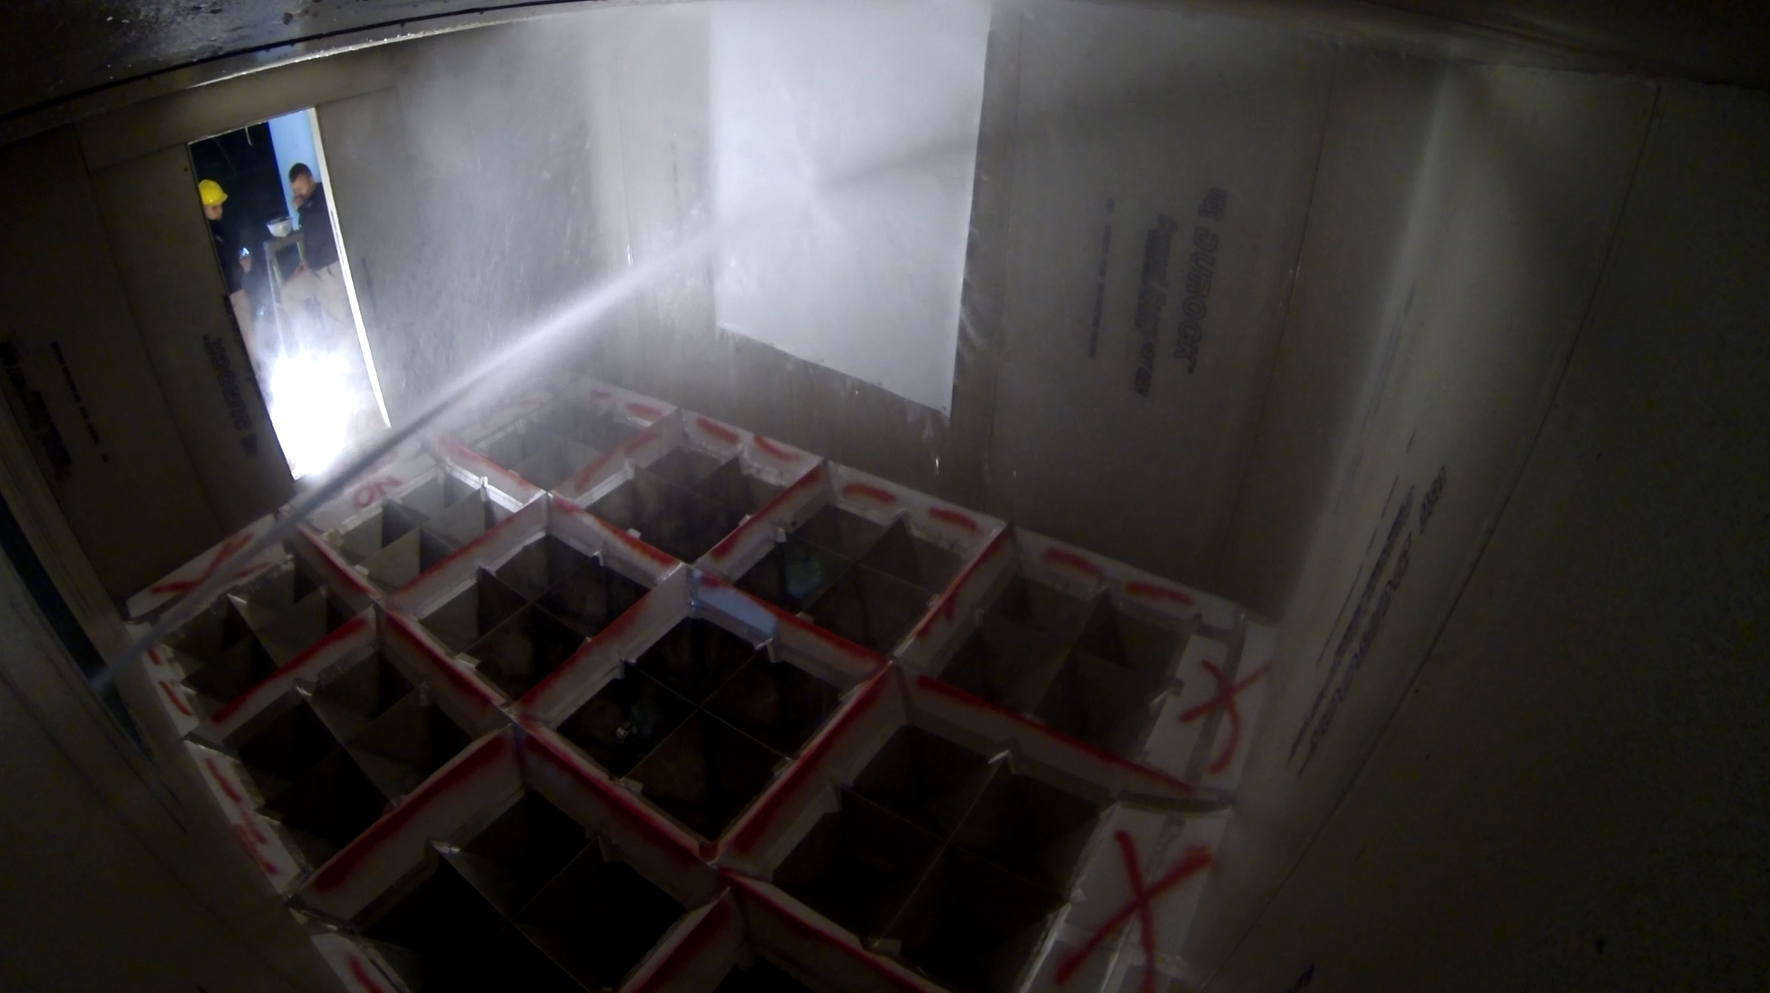
\includegraphics[width=\textwidth]{Figures/Water_Distribution/Nozzle_Directions/Exterior_AtWall_SB.png}
% \caption{Water dispersion of straight stream impacting a wall at an approximate 90$^\circ$ angle}
% \label{fig:at_wall}
% \end{figure}

\newpage

\begin{appendix}

\chapter*{Appendix A - Tech Panel E-Mails}
\label{panel_responses}
\addcontentsline{toc}{chapter}{\nameref{panel_responses}}

\section{Chad Christensen}

Steve,
 
I hope all is well.  I have been swamped with recruit training and trying to finalize our turnout spec. I know I am preaching to the choir when it comes to being busy.  
 
As we continue in in this process for the Fire Attack study one thing have have not gone on record about is the acquired structure burns.  As is everyone else I am very disappointed to know that we will not be conducting those experiments. I think we may be missing an opportunity to gain further buy in from those around the country that see the tests even though just contents fires being tested in actual structures.  We all know the lab houses are real structures too.  Yet with the opportunity to burn in the concrete buildings we can easily recreate the same environment over and over without worrying about it extending on us or getting away from us.  One of the most effective videos for training transitional attack  has been the video NIST not UL (Robin corrected me on that at FDIC last year...ooops) with the side by side room showing how air can push products of combustion not fire. My understanding is that was a contents fire too not a structure fire.  We have not been testing structure fires for the first 24 experiments.  Why don't we continue to test contents fires and do the burns?  I know scheduling is crazy and everyone is busy. Just my thoughts and open for discussion between us.  It would allow an opportunity to test different transitional attack methods(flow pause flow pause/ or flow for 10 sec, 20 sec and so on.)  Again just my thoughts and I don't have all the info I am sure with what is needed for you guys to pull of an acquired structure burn in Columbia.   
 
As for the water mapping portion of the study.  Very interesting results.  So I am curious as to what kind of input you are looking for from us.  As I go through the data the biggest things that stick out to me are: 
1 the smooth bore and straight stream are close in effectiveness and that is great because it can be at the choice of the user as to which nozzle they choose. 
2. the steeper the angle you take the more coverage of surfaces you get which will then give you better cooling when applying water from an exterior position.  Along with a better distribution of water if from a fixed position if from the exterior.  
 
These are all things I feel we have been able to see prior to the study from use on the fire ground or training fires. Now we have the data to support or explain what we see.  This will be excellent for reinforcing particulars in the tactical considerations down the road.  To me and I know you know this. It is that this piece by itself is helpful for the fire-ground but it needs the air entertainment to truly go with it side by side.  Air can so negatively effect the fire ground that if it isn't side by side we could make a bad decision and use a fog stream because it effectively covers surfaces. 
 
Below are some questions I put up on the board last year.  Not sure if you guys have the answers to them yet.  I would like to hear your thoughts to them.  I have a few more points that I am digging into a little more and will email you shortly on those items. If you need more input on water mapping please let me know.  
 
 
\begin{enumerate}
\item Is their any CO data for test 3? It says the sensors were not used? Is the data just not loaded yet or was that the burn they were having sensor issues. Sorry can't remember!

\item If I am reviewing things with an open mind and trying to be objective am I correct in that the temps with door control incorporated drop at a quicker rate than without? Between test 2 and 3?

\item Overall it also appears that water on the fire regardless of how it was applied improved conditions in the fire room and surrounding areas. Yet the straight stream seems to be most effective. Early water on the fire appears to be best for the victims inside.

\item CO levels have been a big concern with guys when it comes to door control. Unless I am missing something it seems at least in my first glance, that CO levels in the survivable space are not raising until suppression? Are we making things worse by putting out the fire? It also seems that with door control CO levels didn't rise any more than without?

\item To determine the best flow type is the velocity what we should be looking at?

\end{enumerate}
 
Thanks
 
Chad
 
Chad Christensen \\
Fire Captain \\
Los Angeles County Fire Department \\
Fire Station 18-C \\
310-671-5368 work \\
951-285-3001 cell \\

\section{Kelly Hanink}

Steve,
 
I have reviewed the report.  One general comment is that I found typos, grammatical mistakes, and awkwardly worded statements that need some general editing.  I would be happy to make those markups and provide if that would be helpful.  But I didn't spend the time doing that up front in case that's something that someone is still set to do at the end.  I believed my objective for you was to read for content and ignore those issues.  I'm one of an odd sort in engineering who actually learned something in English class too. So if you need that basic editing, let me know.
 
As far as content goes, I think the report turned out well.  The description of what happens seems clear to me, and the conclusions follow from that.  I think I can see where people's arguments are going to stem with this information, but then once I think I have that figured out someone comes up with something new.  
 
Anyway, I do have a few items that struck me in terms of content presentation:
 
Figure 5.1 (pg 48) and its associated write-up don't seem to connect exactly.  I had to re-read that piece and look at the picture again to understand it.  The text states that the dispersion was fairly equally radially to 360 deg with some impact by gravity.  But the horizontal arrows (at 90 and 270 deg) are nearly the same as the downward one (280 deg).  I just think the arrows need to be depicted a little more accurately to match the words.
 
When I read the write-up about Figure 5.2 (pg 49) I thought it was lacking info, which it turns out I found in the section on water distribution in the next section.  I don't know if it would be helpful to add text to the water dispersion paragraph to tell the reader about the additional effects of the high angle attack that are described further in the water distribution section or not.  That might not be a thing needed in a research report.
 
I feel like the last two rows Table 5.1 (Tactical Choices Summary) present issues.  The Nozzle Movement tactical choice states a positive impact for Interior attack from an 'O' pattern at the ceiling.  But the prior discussion about nozzle movement says "When compared to each other, nozzle movement had little effect on the distribution in the compartment....While the distribution for the fixed pattern was more uniform (flatter)..."  Those statements don't appear to match.  Further, in the nozzle movement discussion section, there doesn't seem to be any mention of nozzle movement and fog nozzles or any graphs that support the statement in the summary table that an O pattern provides good distribution.  Or if there is, I didn't make the connection very well so you might want to look to see where things might be restated or tied together better.  In the Bale Position section, I don't think it's stated that the testing was only tested in the exterior case.  Maybe that should be added to help with clarity and completeness and to support the last row of the summary table?  
 
I think that's it.  I feel like I haven't been nearly as helpful or as engaged as I wanted to be.  I hope that I can do better at least with the phases that remain and beyond.
 
Let me know if you have any questions about any of my comments.
 
Thanks,
Kelly
 
 
Kelly Hanink \\
Assistant Chief of Health \& Safety \\
Eden Prairie Fire Department \\

Cell: 952.946.9951 \\
Office: 952.949.8356 \\

\section{Josh Hummel}

Report looks good to me.  The larger considerations and pulling all of the concepts together will be on the training end of things.  It obviously all gets weighed against the air entrainment results.  Hope I'm not missing major stuff that others may have seen but it all looked appropriate to me. 
 
I think it's important to include that these findings are purely distribution and not considering air entrainment so conclusions are drawn prematurely by those reading the study.  (This could include the 1/2 bale smoothbore technique discussed at the end or even changing the angle of the stream in the window as it relates to air entrainment.  I'm not sure if these were all tested in the entrainment piece or not)  I can say that I wouldn't have drawn those conclusions as I'm reading the report for what it is, but could see it being a potential issue as you guys know all too well from the spin that gets put on every word coming out of your mouths.
 
Only things I saw were a few spelling things that you all may have noted already but I'm anal retentive soooo... 
`bale' of a nozzle instead of `bail' (changed back and forth throughout)
Freeman is referenced as Freedman occasionally
 
Looking forward to seeing the air entrainment results.  Robin said they'd probably be coming shortly after comments on this report.

\makebox[\linewidth]{\rule{\textwidth}{0.4pt}}

I don't know what the conversations have been to the point with you and Dennis, but obviously I received his email.  I agree with many of the elements he thought were interesting as noted in the PDF he supplied.  Not sure if we were supposed to include those things if you wanted them emphasized in the report at all.
 
I understand the necessity of data on water on the fire from inside the compartment.  It's been a point of discussion from the very first meeting and rightfully so as the past study information has been wildly misinterpreted.  However, to me the water mapping and even the air entrainment to a large extent is about the approach to the fire room.  
 
John Chubb broke down the fire attack in three portions:  deploying the line, approach to the fire room, and extinguishment at/in the room. The second segment is where most of us differ and is where this portion of the project falls.  Once we're in the room the water disperses largely where we focus the nozzle, thus the focus on appropriate nozzle techniques by many of the instructors on the panel.  Water movement in angles not tested in the study have to be extrapolated from the findings as every single angle/pressure/flow/movement can't be tested, however it seems the only truly non-tested element in the water mapping seems like it would be water perpendicular to the ceiling in an effort to disperse in multiple directions.  It's already been acknowledged that a future project is expanding on these projects to determine flow of water across the ceiling in larger spaces which would be the other large difference once inside a large room.
 
I'm assuming you guys know this already or feel something similar.  The assertion that we've missed the mark on the testing, especially in this portion, ironically misses the mark itself.  The work done on this project is quality and certainly gives us a more complete picture of what's happening during the interior attack process.  You, Robin, and the whole group seem to not be impact by the critics too much but I wanted to provide a counter argument saying that I believe the tests were not lacking as otherwise argued.  

\section{Dennis Legear}

Steve and Robin:

Below via the drop box link is a scanned copy of the Water Mapping PDF with my hand written notes on it. Steve you know I wanted to go to the water mapping experiments as I have spent a lot of time over my career messing with this concept.

\hyperlink{https://www.dropbox.com/sh/1wmpqxr2a5fow0c/AAB1bfG-yKjGBKFCOlRtaYDya?dl=0}{Dropbox Link}

Please take the time to review my notes on the scanned copy I took the time to read the entire document.  First the positive, I found the no difference between nozzle pressure and distribution a nice confirmation of a sticking point I have with some.  Also that in a residential compartment probably nothing is gained by an exterior 2.5-inch handline 265gpm+ when it is flown from exterior to interior more water into the room sure, but in the exact same place. (less than 400 sq feet compartment)

\textbf{\ul{Now as for the interior attack part, what was done at the water mapping was not an interior attack.}}  It was a interior approach with water flow from before the threshold of the fire compartment.  I find it valuable, however a interior attack is finished with the nozzle in the fire compartment.  This at best is 1/2 a \ul{interior attack}. 

\textbf{\ul{I have a video attached pieces of what I sent to the ULFRSI to define interior attack.}}  Note the flowing approach (which is what the water mapping interior experiment operations is replicating, remote water to cool) and then the nozzles' entry into the "fire compartment".  At the 40sec mark in the attached video see nozzle past the door threshold at the 1:30 mark hear me yelling \textbf{\ul{through the door!}}  I was reinforcing to the students, one must get up and past through the door to properly wet the entire space of the fire compartment.   This was the student's second try at the flowing push.  Only after the nozzle has passed into the fire compartment do you really own the space as far as application of water to the dry side and directly over head (door header block this on approach), a nozzle in the fire compartment (at critical flow) is sole requirement of a successful interior attack.  These full room wetting actions are impossible from the exterior/interior hallway position or outside the door, remote application.  \textbf{\ul{That exterior flow from the hallway is to permit taking the door way, that is all.}} 

I suggest strongly to re-title the document to \textbf{\ul{Exterior Remote Application and Interior Remote Application Water Mapping}} as that is what it is.  Anyone that reads this with fire duty under their belts will come to the same conclusion, in my opinion.  I have never since 1993 every receive instruction to stop short of the fire room, this experiment in my mind shows what happens when you stretch short by a few feet before the fire compartment.  A failure to be able to gain full access to apply water to the entire fire compartment.    

Now I will be gone from 2/19 till 3/23 out of the country.  I discussed all this with the CC'd members of the panel.  Which are the ones I interacted with the most  (I want this shared with all panel members though).  They to my understanding have the same/similar concerns.  

We all also feel that we would like to have you send out a sample of your analysis of two experiments.  \textbf{\ul{To be frank I was overwhelmed could you please send your thoughts on Experiment \#8 Interior vs  Experiment \#20 exterior.}}  

I picked those two as they are the two bedroom fire examples.  Because again as these members are aware it was decided to stick the nozzle through the window without consulting the panel on many of the exterior fire attack tests.  \textbf{\ul{I/We gave up the second story to gain more experiments, but it was stated no nozzle through the window, stick with Governor Island Approaches.}}  

In fact I have no problem with this (nozzle through the window) and instruct that if you apply water through a first story window for what ever reason required it.  After application if possible reach in and coat the room with water hence gaining the sill and getting a interior attack water application.  I am curious what the other CC'd members think?  But in many ways the nozzle at the UL burns through the window had better ability to coat the fire room because of the probes at the end of the hallway, another point that I took issue with.  The hallway door probes were preventing the nozzle team's direct advancement into the fire compartment hence it was not a good interior gold standard attack.   

\textbf{\ul{The issues above I thought would clearly be resolved at the acquired structure burns.}}  Finally note the One Size Does Not fit All transitional attack doc and the Peach Fire video in the drop box link please review .  This "Peach Street" engine company in the video stretched the 1st handline past the closer stairway that leads to the interior 2nd floor apartment door.  They went to the C side to Governor Island style exterior attack.  They picked exterior water over rapid interior water.  I believe the video speaks for itself.  \textbf{\ul{Why did the exterior water fail to change conditions and the fire continue to grow?  Can you provide your thoughts on this video Steve and Robin?}}  

I did wrote this because I have a feeling I will miss the last meeting based on my request for firm dates over the last few months.  Loss of the acquired structure burns where void space spread, and regrowth could have been better quantified was a big impact to this projects ability to succeed.  I suggest applying for another grant and moving forward in the future.  \textbf{\ul{As of now I feel we have missed the mark for whatever reason maybe we did not properly define Interior attack to UL staff,}} because a nozzle through a window is now interior attack for example.  The very reason I was adamant not to allow it, was not because I would not do it or have not done it, but because it is not an exterior attack.  An interior attack is one were the nozzle is in the fire compartment at the end and can coat the entire room with water.  These are my thoughts I still hope to make the final panel meeting.  
Thanks in advance,

Dennis 925-787-6875

\section{Jordan Mohr}

Steve,
 
Everything that I can see from my point of view for the water mapping looks good. The explanation for how the results were recorded, the visual charts and the brief history of how we got to this point really helps the reader understand why these tests were done. I think it was well put together and knowing that this is just a small piece will be beneficial. Personally I feel like newer members to the fire service like myself will be able to understand this and benefit from it in conjunction with our other results.
 
Thanks
316-259-3135
 
Jordan Mohr | Firefighter | Sedgwick County Fire District \#1 \\
p: (316) 660-3433 | f: (316) 660-4443 | Jordan.Mohr@sedgwick.gov \\
7750 N Wild West Dr | Park City, KS 67147|www.sedgwickcounty.org \\

\section{Jerry Knapp}

Steve,
 
First, another piece of magnificent research!!  
 
The data was not surprising and in general, what i anticipated from observing fire streams in buildings. Since a majority of the water ends up near the wall-floor area it would appear that these fire streams should not be effective.  However, if we recall that we are evaluating only residential occupancies it may make perfect sense.  In residences, furniture, TVs, sofas, etc are generally not in the center of the room but near the walls.  This geometry obviously allows occupants to move freely thru the space.  
 
Further, as the nozzleman, during an interior attack, moves his stream in the O,T,Z or U pattern he is directing water on the fuel at some point during that movement with associated stream break up resulting in water falling on other fuel in the room.  On page 20 of the draft, if i understand the data correctly, the smooth bore "O" pattern nozzle movement yielded more buckets that exceeded 0.05gpm/ft2 which may be the reason for it's practical success in the field(?).
 
 hose that i call "the wild whippers" that advocate violent movements of the nozzle seem to be causing the stream to break up and possibly fall onto the fuel long before the stream is broken up on the far wall or ceiling.  This violent nozzle movement may result in water falling directly on the fuel at great cost of muscular-mechanical effort of the nozzleman.
 
As always i am reluctant to comment on the draft because of the amount of data collected and my inability to process it into some sensible form.  As you always state we should be hesitant to draw conclusions without evaluation of the complete volume of data.  Regardless, this study has put real numbers to what we all "think and know" from our experience which is a huge benefit to our Fire Service.
 
Please keep up the good work.
 
Respectfully,
 
Jerry Knapp

\section{Hans Neiling}

Hi Steve,
 
Here are my comments or observations on the water mapping research. Reading through the report you guys made my overall opinion is that there are not much differences between all of the experiments. There are some small differences between the different type of nozzles and pressures, flow rates and fog pattern. But than we talk about nuts and bolts, a couple gallon more in the back or left side of the room? To me this test tells me more about how the water is being spread inside the room and it really doesn't matter how you apply it, as long it's getting in that room of fire and as quick as possible. The end result will remain the same, a knockdown and it gives us time to enter en overhaul :) without getting ourselves in too dangerous situations.
 
In the reports it talks about a narrow fog that would cover the window entirely, for water mapping I can guess why this test is done, but looking at the transitional attack itself that would be the wrong nozzle setting to apply this technic? we don't want to close that window with a water pattern correct? so why was chosen for this nozzle angle and not just a angle a bit smaller that would not cover but lets say blocks only 50\% of the opening?
 
As I said before I'm happy to see these results and surely that there's not much difference between them all, which gives me a good feeling when applying water from the outside that it does the job quickly.

Would love to see these tests with actual fire and measure what kills the fire? steam or water? to me it's a 75\% steam and 25\% cooling by the water, a gut feeling :)
 
looking forward to the next report :)
 

Hans Nieling \\
Co-owner / Instructor CFBT-nl \\
tel; 06 14 45 18 49 \\

\section{Jason Floyd}

Steve, 

I apologize for my tardiness. I had Friday, February 17 as the due date in my calendar.
 
My overall summation of the water mapping is one of surprise and enlightenment. What I ``thought I was achieving on the fireground'' and have been preaching is far different from the reality the experiments proved.
 
I don't have any real concerns regarding the experiment methodology or design. I have included some edits and questions below. I feel confident this is the first in a series of tests that will explore where our water goes. This project was a great start!
 
The droplet fallout which I perceived to assist with suppressing burning materials throughout a compartment was less evident. I have been clinging to the work done by Vestal/Bridge for years to draw this conclusion. This has also promoted additional concerns regarding the efficiency of transitional attack. The gas cooling may be shorter lived since the burning materials have not been effectively treated. Reflex time for interior attack cannot be underestimated.
 
The nuggets I can take away immediately from this project are the guidance on the steep to shallow angle and the half bale for better distribution.
 
Although the water riding along the ceiling and down the back wall appears negative as it relates to distribution. I believe it might be determined later under live fire to be positive as it relates to gas cooling given the longer interaction at upper levels.

Future Research Needs \\
Many of us on the panel are practitioners of `hit and move/flow and move' suppression techniques.
\begin{itemize}
\item Hit and Move/Flow and move streams would impact the hallway ceiling in advance of the fire compartment. The technique we use locally includes treating the leading edge of the fire gases at a steep angle and progressively working the stream to a shallow angle towards the fire compartment. 
\item Based on the dispersion demonstrated in the experiments it appears that a hallway configuration with an approaching stream would yield center distribution. 
\end{itemize}

How can we achieve center room distribution?
\begin{itemize}
	\item Obviously, the soffit attack needs additional examination.
	\item The mid-level collision with a surface prior to the ceiling creates a fanned-out pattern. This makes sense.
	\item `Lintel attack'
\end{itemize}
 
Edits
\begin{itemize}
\item Table 3.1
	\begin{itemize}
	\item 1 1/4" Tip had a flow rate=260 GPM
		\begin{itemize}
			\item Why was this tip used in place of 1 1/8"?
			\item 1 1/4" tip at 50 PSI should flow 328 GPM.
			\item Should there be further explanation?
		\end{itemize}
	\end{itemize}
\item  Page 18
	\begin{itemize}
		\item 2nd paragraph starts: `distributed.'
	\end{itemize}
\item Page 49, 1st paragraph
	\begin{itemize}
		\item Note that water did not `bounce' of the ceiling and fall into the center collection bins.
	\end{itemize}
\item Page 53, 1st paragraph
	\begin{itemize}
		\item This prevent a direct statistical comparison of interior versus exterior streams.
	\end{itemize}
\item Figures 5.13 and 5.14
	\begin{itemize}
		\item Consider revising the description of the figures to include `full bale' and `half bale'.
	\end{itemize}
\end{itemize}
 
I was genuinely impressed by this component of the project. I must keep focused on the intent of this research and not get ahead of where we are. Thank you for your hard work and dedication.
 
Sincerely,
Jason Floyd

\section{Jake Hoffman}

Gentlemen,

I am very sorry for my tardiness in sending you these notes.  I'm kind of all over the place so hopefully they make some sort of sense. 

Bale Position
Half bale seems to allow for better distribution into the middle of the room but how much air are we introducing?

5.5.3 - Angle of Impact - To kind of add on to nozzle positioning inside vs. outside the target room, would it be worthwhile to put something in the report about how your angle will vary depending on how far you are from the seat of the fire, etc.  While approaching (making the hallway) if you have clear line of sight into the fire room you will most likely have ``Min Angle Ceiling'', effectively throwing most of the water at the far wall.  But once you make your way into the room or are at the doorway, max angle is best to cool all surfaces.

Pg 3 -  ``...cool fuel surfaces to restrict and slow pyrolysis...'' - I am not sure if or how we emphasize this point in our final report, but I feel it is extremely important.  

Even though people talk a big game about putting water on the fire and how we ``used to never put water on smoke...'' In reality, many people are waiting to flow water.  Modern textbooks do a very poor job of emphasizing the importance of this tactic. 

I know that we are providing the data and the purpose of the panel is to guide the experiments using our experience, etc. but I feel that we need to strongly word certain topics such as this when the final report comes out. 

Where we draw the line between data and tactics isn't for me to decide obviously but when it comes to nozzle work and aggression, entering the room to cool all surfaces, etc... these things seem like common knowledge to myself and other panel members, but to most of the fire service might be something they have never heard.

I know water flux is defined on Pg 5 but maybe emphasize so that the reader doesn't have to flip back to check the definition. In burns, nozzle was put ``Into the window'' ... Water mapping was not?

Nozzle Patterns and Water Distribution - We teach ``floor, wall, ceiling'' to our recruits and during a realistic interior attack this would obviously greatly alter the water distribution in the room compared to the experiments.  Data is good, but maybe not 100\% accurate for interior approach/attack. Obviously directing stream at ``floor'' of ADD could have caused damage, hard to replicate in the lab. 

Was surprised to see that changing flow and pressure had no significant effect on distribution, only flux. 

-------------------------------------------------------------------------------------------------------------- \\

I like how Dennis suggest emphasizing in each table the locations that did NOT get 0.05 GPM... I figured it out while reading it no problem, but to firefighters, making it simpler and/or easier to understand quickly will get more buy in

I do NOT agree with Dennis that 1 line should stay exterior to ``monitor regrowth risk unless nozzle can be placed into the window.  ''

A major department in Ohio has tried this ``monitor for regrowth'' and last I knew had proceduralized it to where that first line was required to flow for X \# of seconds and must remain in position to flow again if needed until an interior line is there.  We have tried similar tactics here and the general consensus is that it is a waste of time, manpower, and a line UNLESS normal entry is impeded (hoarder conditions, tough forcible entry, commercial structure, etc).  For us in Toledo, its generally not the regrowth in the fire room that we are most worried about because as we have seen hundreds of times on TFD just in the past year or so, the transition works pretty damn well, but our concern is the fire running the void spaces, knee walls, etc. and you can't put that fire out by waiting outside to monitor for regrowth.

Obviously acquired burns would have addressed this but I realize its not possible so I won't throw a temper tantrum like some.

If we choose to transition the fire, we have put water on the fire and have ``reset'' it.  The best way to ``monitor for regrowth'' is to get inside, put water on the seat, and aggressively check for extension.  

One of the best pieces of advice that I have ever received from a senior man was ``if you want to see more fire than anyone else, make the attic quick.''  

This proves to be true on an almost daily basis and even my fat ass gets into attics because in Toledo, if its more than a contents fire, there will be fire in the attic.  Sorry for the anecdote, but I feel very strongly that leaving a line outside to monitor for regrowth is useless and a waste. (unless entry/advance is impeded as mentioned above)


Sorry again for not having these submitted on time and sorry for the rambling.

Jake

\section{Ray McCormack}

Comments on Testing
Ray McCormack

I can see where the nozzle teams non entry of the fire room during live fire testing closely replicated the Water Mapping tests. In addition the exterior portion of the ``transitional attack'' was vastly different then previous definitions with nozzle penetration of the fire room.

While we can't change the data or test formats used we must be mindful of accurately reporting test parameter and their results and how they impact the fire service with their extinguishments. While the interior attacks didn't end inside the fire room which is uncommon neither did the interior portion of the ``transitional attacks''.  

I do know that there was no fire regrowth once water entered the room from the doorway, proving the effectiveness of stream movement from an interior position. Utilizing a variation of this effect was the placement of the nozzle into the room from the exterior which was able to ``center'' on the burning seat of the fire

What I believe we need is clarification on the variable where the nozzle is being placed inside the fire room during exterior fire attack. This is a variation of a ``transitional attack''. This variation apparently grew out of the Water Mapping results that showed how the rooms center was not being hit with water. So this addition placement replicated what an interior line can do. Then the question is, did we actually test ``transitional attack'' or some limited hybrid version of it?

What I have seen from the ``transitional attack'' tests is a time sensitive situation and added stress to a single lines mobility/capability. Time sensitive on several accounts, one being the amount of time the water is applied and the time it takes to move that line to the entry door and enter. This impact will differ in the real world due to many factors such as window placement, room shape, stream application method, shape, and distance. I believe the effectiveness of exterior attack at greater heights with a hand line will also diminish as the stream breaks up outside of the target entry area and occludes more of the intended opening. 

I believe the added kicker (nozzle in room) was needed for the exterior attacks to thwart the fire from rebounding during the tests. Exterior water during ``transitional attack'' only seems to result in fire knock back. Without the stream being placed inside the room fire knockdown wouldn't have been achieved. This issue is compounded when that hoseline is being shared between two spaces as in a ``transitional attack''.

The difference between knock back and knockdown is, you have a fire that appears to be down only to quickly regrow (knock back) and one where regrowth is further stunted (fire knockdown). The knock back state is common during the exterior attack due to a lack of nozzle movement that is low enough to hit base fire and the rooms center which equates to ineffective stream placement and non extinguishment.

A fire that is knocked down is in it's closest state to extinguishment. This state was achieved from the room entry point on all tests which was quickly followed by extinguishment. 

An analogy could be made of an engine attacking a kitchen fire where the cabinets are going, and a limited spray of water is applied (knock back) and you concluded operations only to find as you walk away that the fire is back. You wouldn't last long as a company officer of that company. Fires that are in a knockdown state can also regrow, however their redevelopment is typically stalled or finalized due to enhanced water placement and or duration and being able to effectively manipulate your hose stream, something that is typically denied from the buildings exterior.

If you're going to use exterior attack then use it correctly. Meaning don't move the line from the point of water entry. Keep it in place so it can hit the fire again when needed. When a fire regrows after exterior water is applied in a ``transitional attack'' then we haven't solved the problem we have just shifted it to the interior.  

Without a separate standby exterior stream at the ready we will be allowing the same event were trying to stop in the first place to occur again. If we vigorously applaud half measures of extinguishment such as ``transitional attack'' as the cure then we risk applying measures that are even less effective in the real world due to additional conditions encountered. 

Yes ``transitional attack'' is a half measure. Only a portion of the fire issue has been dealt with and it's effect is temporary. The exterior attack provides knock back only the interior portion provides knockdown and full extinguishment. If interior attack in some form is not undertaken then exterior attack limitations will rear their ugly head in the form of fire regrowth, non extinguishment and fire spread.

Seven of the experiments in this study were ``transitional attack'' and this fire attack method is implemented in various forms throughout the country, our job is to better define it, and apply the proper operational warnings of its application limitations and limited effectiveness.

If you find that exterior attack is inadequate in fire knockdown without placing the nozzle into the interior space through the window then that information must be publicly shared.

If you tell people that if you quickly bounce from exterior attack to interior attack without another line in place to control fire regrowth then you are giving out a false narrative of extinguishment via ``transitional attack''. 

When the fire regrows after an exterior hit it is no longer a ``transitional attack'' because it has now retransitioned to an interior attack until such time exterior water is reapplied. When the exterior first half of ``transitional attack'' doesn't accomplish knockdown then we are obligated to inform the fire service of this serious limitation.

One of the tests involved a bedroom (video included) close to the entry door, when a closet door failed in that room it opened up a void that lead to vertical spread through the roof. That fire was a classic example of giving the room close to the building entrance door a quick exterior hit before going in. There was no nozzle insertion into the fire room. A standard ``transitional attack'' was initiated from the exterior and the line was repositioned to the entry door. The fire rebounded to original intensity as the nozzle team entered. We can debate why this happened but the real world implication is that it did happen.

Are we going to extoll the use of a tactic if it's usefulness or limitations aren't well defined? The most common outcome of a ``transitional attack'' creates a temporary drop in temperatures, fire gas growth, and semi delayed fire rebound. The risk is unchecked fire regrowth and increased risk to the interior attack team who are operating under rapidly redeveloping and changing fire conditions. 

Once that line goes inside what is the role does the back up line? Where is it positioned? We never get the whole picture of a fire or it's spread from the exterior. We do not gain extinguishment or the ability to extinguish without entry and attempting to put it all on one handline without selecting a placement for a back up line is a consideration the fire service needs to address when utilizing ``transitional attack''.

Sincerely
Ray McCormack

\section{Samuel Hittle}

Can you please provide me with the ANOVA data results for the repeatability of water mapping? Thank you.

Samuel Hittle \\
Wichita Fire \\
316-992-2997 \\
Traditions Training Instructor \\
www.traditionstraining.com  \\
shittle@traditionstraining.com \\

\section{Dan Doyle}

Steve, UL Staff, and Panel Members,
 
 
First, I hope this email finds everyone well.  It's been sometime since we've all been together and we are finally getting to process some of the information in a constructive way.  Although it is somewhat tough to feel your way through, the info is now being feed and processed by analyzing it piece by piece.  
 
Second, before I get into my thoughts from the information process there is a main component that seems to get lost in discussion.  That is the victim packages.  While we are processing water mapping right now, the burns showed some interesting findings as to how the victim packages responded in Chicago.  The main focus for me is what quickens my time to victim contact? Does my stream, pattern of delivery, or type of push (Flow \& move / Hit \& move), positively impact the victim and reduce time to contact/rescue.  We can not lose focus on that subject as it is a driving force for this study and the heart and soul of the fire service.  In researching that, we have an opportunity to clarify a few things as it pertains to stream selection, application, push type, or type of initial attack.
 
So getting into the meat and potatoes of the email, a modification was brought up that occurred while we were in attendance in Chicago.  The nozzle penetrating the window after initial flow.  The bail was backed down and the nozzle was pushed into the window and thrashed around a bit before repositioning to the front door.  Once repositioned, the team then pushed into the structure and down to just short of the fire room. (As I understand it the nozzle was commonly past around at the sensors at the door but only a foot to accomplish total knock down!)  We will come back to the ``Knock down'' comment in a minute.  This is where time and realism come into effect for me.  That ``transition'' from the window frame to the front door encompasses moving the entire system inline with the door to now ``make the push'' to final knock down. While UL accounted for the time difference pausing before entering the door.  This did NOT account for the FATIGUE issue.  In fact it gave the crew a chance to catch their breath and gather themselves before entering!  There were ZERO obstructions to maneuver around.  (Bushes, mailboxes, front porches, steps, fences, gates, cars, ditches, hills, dogs, ferrel cat...  I can go on!)  All of this contributes to crew fatigue.  It then slows that final push and TIME TO VICTIM CONTACT.  You may be a Crossfit guru or a donut eating dinosaur, either way task execution on this job creates fatigue quickly.  ``Work Smarter Not Harder''
 
Some of the same obstructions would also hinder you from getting right up into the window to get the nozzle in!  I feel that the adjustment may have benefited the ``Transitional Style'' attack by NOT allowing substantial regrowth. (Which was seen in the the transitional hits prior to the window penetration) However, the application for this adjustment is extremely minimal in its practicality.  You have now reduced the opportunity for use down to an easily reachable window on the first floor.  
 
Most of the fires that Pittsburgh responds to are typically above the first floor or if they are on the first floor the urban environment doesn't really lean itself to accessibility.  While I have a vested interest it the way my employer does business, I do realize that we are addressing the fire service as a whole.  Response dynamics, namely staffing come into play here.  
 
 
Let's return to the ``Knockdown'' comment above.  During the burns we were informed that the nozzle did in fact enter the room but only a reachable distance past the sensors.  Then after the scenario was complete everything was wet down for removal.  This is an issue as it pertains to the water mapping accuracy.  One of the main points that our group teaches is the ``Four Corners Rule.''  This rule applies when extinguishing a room of fire and especially if you have to operate past a room that was ``knocked'' to get to another involved room.  The flow of water during the approach of the room, then doorway,  room penetration, then all four corners.  This is done quickly due to additional fire but the room is hit in its entirety before moving on.  (Keep in mind we are not camping out in the room but making sure nothing will come back at us after we move forward.)  If the nozzle doesn't get past the threshold of the door that is no different than hitting the room through a window and only covering one wall.  (Most of us would chock that up as a fail because you stretched short!)  If the room is not finished off during the interior push all you have accomplished is an incomplete ``Transitional attack via the Interior!''
 
While I know we are analyzing the water mapping results right now all of the discussed factors play a huge part.  The Main reason I took the time to elaborate on the above observations and concerns is that the interior portion of the water mapping is NOT indicative of an interior attack in any stretch of the imagination!  I read over the information multiple times to see if I was missing something but... Finally realized that I was not!  The stream coming from the interior ``Mounted'' line regardless of nozzle choice never hit below waist height or the floor.  If a crew was approaching that room both the right and left walls would have been pounded by the crews stream along with the ceiling and FLOOR.  The end of the hallway, the threshold of the door, and the room upon penetration, would all have been beaten by the crews stream.  Now I know that we all do business a bit different on the interior but I'm confident we aren't that far off.  AT NO POINT DID THE STREAM HIT THE FLOOR OR AN AREA WHERE CONTENTS WOULD HAVE BEEN.  I also realize that the floor was not able to hold contents.  Thats not my issue here.  If you look at the graphs the feedback was almost the same exterior to interior unless the angle of delivery changed.  In my personal opinion the interior portion of the water mapping is completely invalid and should not be utilized.  In fact comparatively, I believe that it is inappropriate to use the information on hand, having to generate more language than we already have to explain the indifference. 
 
The reader reviewing the published final results or someone sitting in a class on this prior to our final wording decision could easily be mislead with information that really doesn't apply in a reality based interior attack.  
 
I'm not exactly sure what lead to applying water unrealistically, it could have been shotty construction that got lit up by a pressurized stream or the mapping grid not holding the weight of a crew or a nozzle firefighter.  If any of these were the case then we should have stopped rethought, reconstructed and moved on.  I haven't heard a reason for it but feel like we need one.  
 
While my comments above may seem convicting they are not meant to be that way.  The work and considerable time that is put into these concepts is incredible but it also needs to be extremely realistic, and provide steadfast proven information.  While theres some info to be processed I think we came up short of the room on this one...
 
Thank you,
 
Dan Doyle

\end{appendix}

\end{document}